\documentclass[conference,onecolumn]{IEEEtran}
\usepackage{cite}
\usepackage{amsmath,amssymb,amsfonts}
\usepackage{graphicx}
\usepackage{textcomp}
\usepackage{xcolor}
\usepackage{booktabs,array}
\usepackage{newtxtext,newtxmath}
\usepackage{url}
\usepackage[hidelinks]{hyperref}
\usepackage{tikz}
\usetikzlibrary{arrows.meta,positioning,fit}
\graphicspath{{figures/}}
\newcommand{\KiB}{\,\mathrm{KiB}}
\newcommand{\MiB}{\,\mathrm{MiB}}
\newcommand{\codeurl}{https://github.com/mahaswint/cs5290/tree/main/pim-reproduction}
\title{Contribution Results: Indexed Retention, Slabs and Pinned Metadata}
\author{\IEEEauthorblockN{CS5290 Project Group}}\begin{document}\maketitle
\section{Progressive mechanisms}
IA/IF add indexed lists and ownership lookup with adaptive-64/fixed-2 retention. SA/SF add 64 KiB MRAM spans for 2049--4096 B requests. PA/PF additionally pin a 528 B upper buddy prefix in WRAM, costing a measured 540 B endpoint increase. Payload heap, input and empty-byte budget are equal within each comparison.
\begin{table}[!htbp]
\caption{Final work runtime (milliseconds) for every stage on five complementary cases.}\label{tab:final-main}
\centering\small
\begin{tabular}{lrrrrrrr}\toprule
Case & B & IA & IF & SA & SF & PA & PF \\ \midrule
Larson 8--4095 B (4T) & 160.089 & 164.537 & 159.826 & 24.026 & 19.894 & 19.172 & 16.255 \\
CloudPhysics cache (4T) & 122.773 & 122.925 & 122.784 & 114.586 & 114.528 & 113.023 & 113.075 \\
Larson 8--8191 B (4T) & 320.457 & 342.572 & 331.666 & 216.369 & 232.613 & 204.807 & 188.202 \\
Gowalla churn (4T) & 148.847 & 26.172 & 24.961 & 26.918 & 25.830 & 26.954 & 25.827 \\
PrIM selection (4T) & 14.134 & 14.180 & 14.180 & 14.135 & 14.135 & 14.133 & 14.133 \\
\bottomrule\end{tabular}
\par\vspace{2pt}{\footnotesize B: scan fixed-2; I: indexed; S: indexed plus 64 KiB slabs; P: indexed plus slabs plus pinned metadata. A uses adaptive interval 64; F retains at most two empty spans/class. All rows use four tasklets.}
\end{table}

\begin{table}[!htbp]
\caption{Final paper-derived cases: the baseline and both full-stack policies.}\label{tab:paper-final}
\centering\small
\begin{tabular}{lrrrrrr}\toprule
Case & B work (ms) & PA work (ms) & PF work (ms) & PA speedup & PF speedup & PF total speedup \\ \midrule
Gowalla linked blocks (4T) & 19.330 & 15.479 & 15.198 & 1.249 & 1.272 & 1.335 \\
Gowalla growing arrays (4T) & 5.752 & 5.845 & 5.494 & 0.984 & 1.047 & 1.070 \\
KV growth replay (4T) & 24.382 & 19.657 & 19.625 & 1.240 & 1.242 & 1.210 \\
32 B microbenchmark (1T) & 0.875 & 1.077 & 0.990 & 0.813 & 0.884 & 0.799 \\
32 B microbenchmark (16T) & 6.938 & 5.719 & 5.648 & 1.213 & 1.228 & 1.105 \\
256 B microbenchmark (1T) & 2.076 & 2.005 & 1.925 & 1.035 & 1.079 & 0.994 \\
256 B microbenchmark (16T) & 34.201 & 27.750 & 27.641 & 1.232 & 1.237 & 1.192 \\
4 KiB microbenchmark (1T) & 20.912 & 1.858 & 1.778 & 11.255 & 11.763 & 1.512 \\
4 KiB microbenchmark (16T) & 508.474 & 22.335 & 22.243 & 22.766 & 22.860 & 6.746 \\
\bottomrule\end{tabular}
\par\vspace{2pt}{\footnotesize Graph cases are reduced ports; KV is an allocation-only replay and excludes attention/serving. Original request sizes and 128 microbenchmark requests/tasklet are retained. Values below one are regressions.}
\end{table}

\begin{figure}[!htbp]
\centering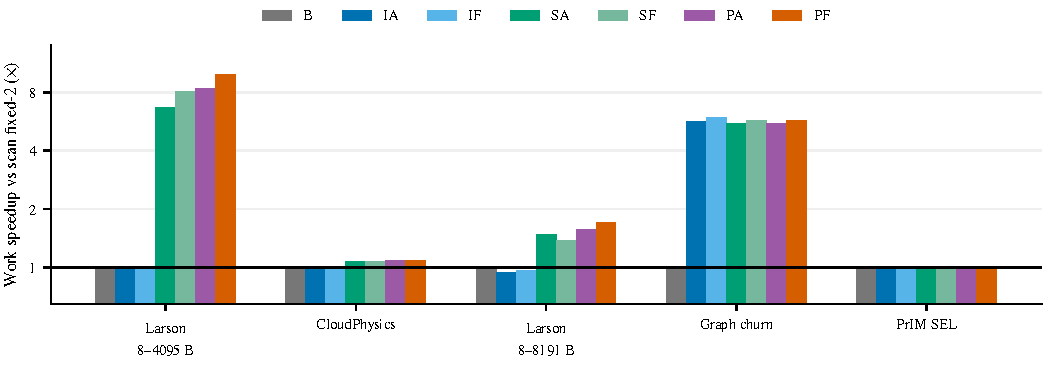
\includegraphics[width=\textwidth]{final-progression.pdf}
\caption{Every requested final stage, at four tasklets.}\label{fig:contrib-progression}
\end{figure}
\begin{figure}[!htbp]
\centering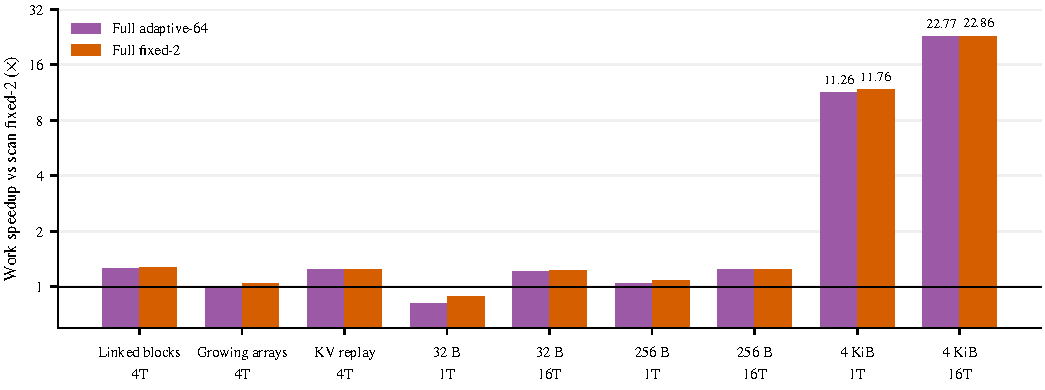
\includegraphics[width=\textwidth]{paper-workloads.pdf}
\caption{All final paper-derived/replay settings, including regressions.}\label{fig:contrib-paper}
\end{figure}

\section{Attribution and costs}
The 4 KiB frontend is new: original classes stop at 2 KiB. The largest slab gains therefore reflect caching a previously uncached size, not evidence that every original class should use bigger pages. Fixed retention is faster on many stable traces. The one-tasklet 32 B case regresses; sparse survivors can reserve 128 KiB for 8 KiB of live payload. Pinning gains below isolate metadata placement with the same slab/policy.
\begin{table}[!htbp]
\caption{Pinning isolated from the slab and retention policy.}\label{tab:pinning}
\centering\small
\begin{tabular}{llrrr}\toprule
Workload (4T) & Policy & Work speedup & Total speedup & DRAM-byte reduction (\%) \\ \midrule
Larson 8--4095 B & A & 1.253 & 1.258 & 48.34 \\
Larson 8--4095 B & F & 1.224 & 1.230 & 46.48 \\
CloudPhysics cache & A & 1.014 & 1.011 & 4.45 \\
CloudPhysics cache & F & 1.013 & 1.010 & 4.44 \\
Larson 8--8191 B & A & 1.056 & 1.193 & 66.92 \\
Larson 8--8191 B & F & 1.236 & 1.208 & 66.49 \\
Gowalla churn & A & 0.999 & 1.169 & 9.66 \\
Gowalla churn & F & 1.000 & 1.164 & 9.66 \\
PrIM selection & A & 1.000 & 1.000 & 0.00 \\
PrIM selection & F & 1.000 & 1.000 & 0.00 \\
\bottomrule\end{tabular}
\par\vspace{2pt}{\footnotesize The pinned variant uses a measured 540 B additional WRAM endpoint in each pair. It is an added-storage comparison, not an equal-WRAM-budget replacement experiment.}
\end{table}

\begin{table}[!htbp]
\caption{Allocation demand, full-execution backend/DRAM activity and peak payload reservation.}\label{tab:traffic}
\centering\small
\setlength{\tabcolsep}{4.5pt}
\begin{tabular}{lrrrrrrr}\toprule
Case & Timed allocs & B buddy & PF buddy & B DRAM MiB & PF DRAM MiB & B peak KiB & PF peak KiB \\ \midrule
Larson 8--4095 B (4T) & 1,024 & 1,416 & 255 & 5.412 & 0.722 & 996 & 1244 \\
CloudPhysics cache (4T) & 150 & 183 & 95 & 5.879 & 5.365 & 1408 & 1596 \\
Larson 8--8191 B (4T) & 1,024 & 1,865 & 1,311 & 10.689 & 2.247 & 1624 & 1932 \\
Gowalla churn (4T) & 3,397 & 360 & 360 & 15.696 & 8.433 & 1440 & 1440 \\
PrIM selection (4T) & 0 & 0 & 0 & 1.876 & 1.939 & 0 & 0 \\
Gowalla linked blocks (4T) & 1,687 & 360 & 360 & 7.289 & 4.409 & 1440 & 1440 \\
Gowalla growing arrays (4T) & 1,690 & 93 & 93 & 1.858 & 1.221 & 372 & 372 \\
KV growth replay (4T) & 1,024 & 220 & 220 & 2.840 & 1.915 & 880 & 880 \\
32 B microbenchmark (1T) & 128 & 2 & 2 & 0.032 & 0.088 & 8 & 8 \\
32 B microbenchmark (16T) & 2,048 & 32 & 32 & 0.456 & 0.414 & 128 & 128 \\
256 B microbenchmark (1T) & 128 & 9 & 9 & 0.114 & 0.148 & 36 & 36 \\
256 B microbenchmark (16T) & 2,048 & 144 & 144 & 1.771 & 1.395 & 576 & 576 \\
4 KiB microbenchmark (1T) & 128 & 128 & 9 & 1.430 & 1.086 & 512 & 576 \\
4 KiB microbenchmark (16T) & 2,048 & 2,048 & 144 & 22.816 & 16.381 & 8192 & 9216 \\
\bottomrule\end{tabular}
\par\vspace{2pt}{\footnotesize Buddy counts and DRAM bytes cover the full execution; they are not timed-work counts. Peak excludes the extra 64 KiB owner map, buddy metadata and identical application tables. DRAM counters exclude WRAM and instruction fetches.}
\end{table}

\begin{figure}[!htbp]
\centering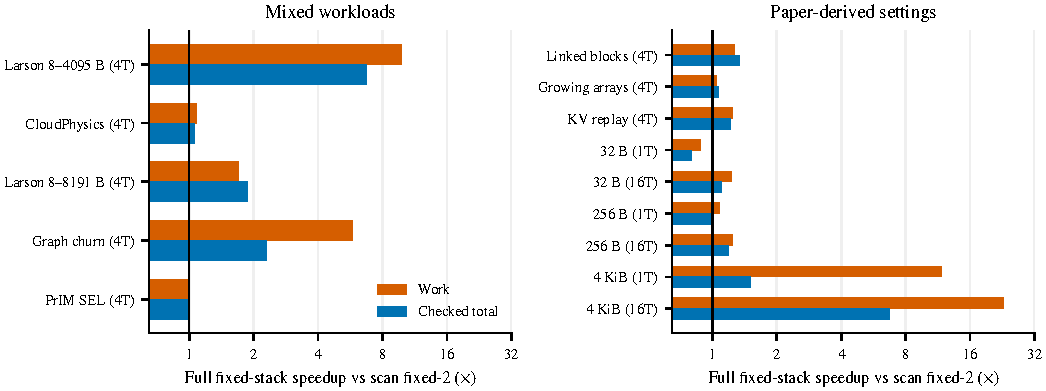
\includegraphics[width=\textwidth]{work-versus-total.pdf}
\caption{Work and checked-lifecycle gains differ.}\label{fig:contrib-total}
\end{figure}

\section{Scope and validation}
The final main comparison has 98 configurations over fourteen settings, all successful. The parent and paper extension audits preserve 47 and 42 native cases respectively. Measurements use a deterministic 350 MHz single-DPU simulator; they do not establish hardware or complete-application throughput. Graphs are reduced Gowalla ports, and KV replay excludes attention and serving. Source, traces, native evidence and simulator hashes are audited.\end{document}
